\documentclass{report}

\usepackage{geometry}
\usepackage{amsmath}
\usepackage{graphicx}
\usepackage{url}

\renewcommand{\bibname}{References}

\graphicspath{ {./images/} }

\title{Furuta Pendulum Control Report}

\author{Samvrit Srinivas}

\date{\today}

\begin{document}

\maketitle

\chapter{Motor Controller} \label{chap:motor_controller}

The input for the furuta pendulum is a torque applied by the motor at the base of the setup. We use a DC brushed motor for this purpose, and hence the motor controller is designed to be a current controller, as the torque is directly proportional to the winding current. The winding current is controlled by applying a pulse-width-modulated voltage at the motor terminals. In the following sections, we will look into the mathematical model and the control design of the current/torque controller.

\section{Mathematical Model}	\label{sec:math_model}

Following represents the current-voltage dynamics of a DC motor \cite{motor_control_umich_lecture}:\\


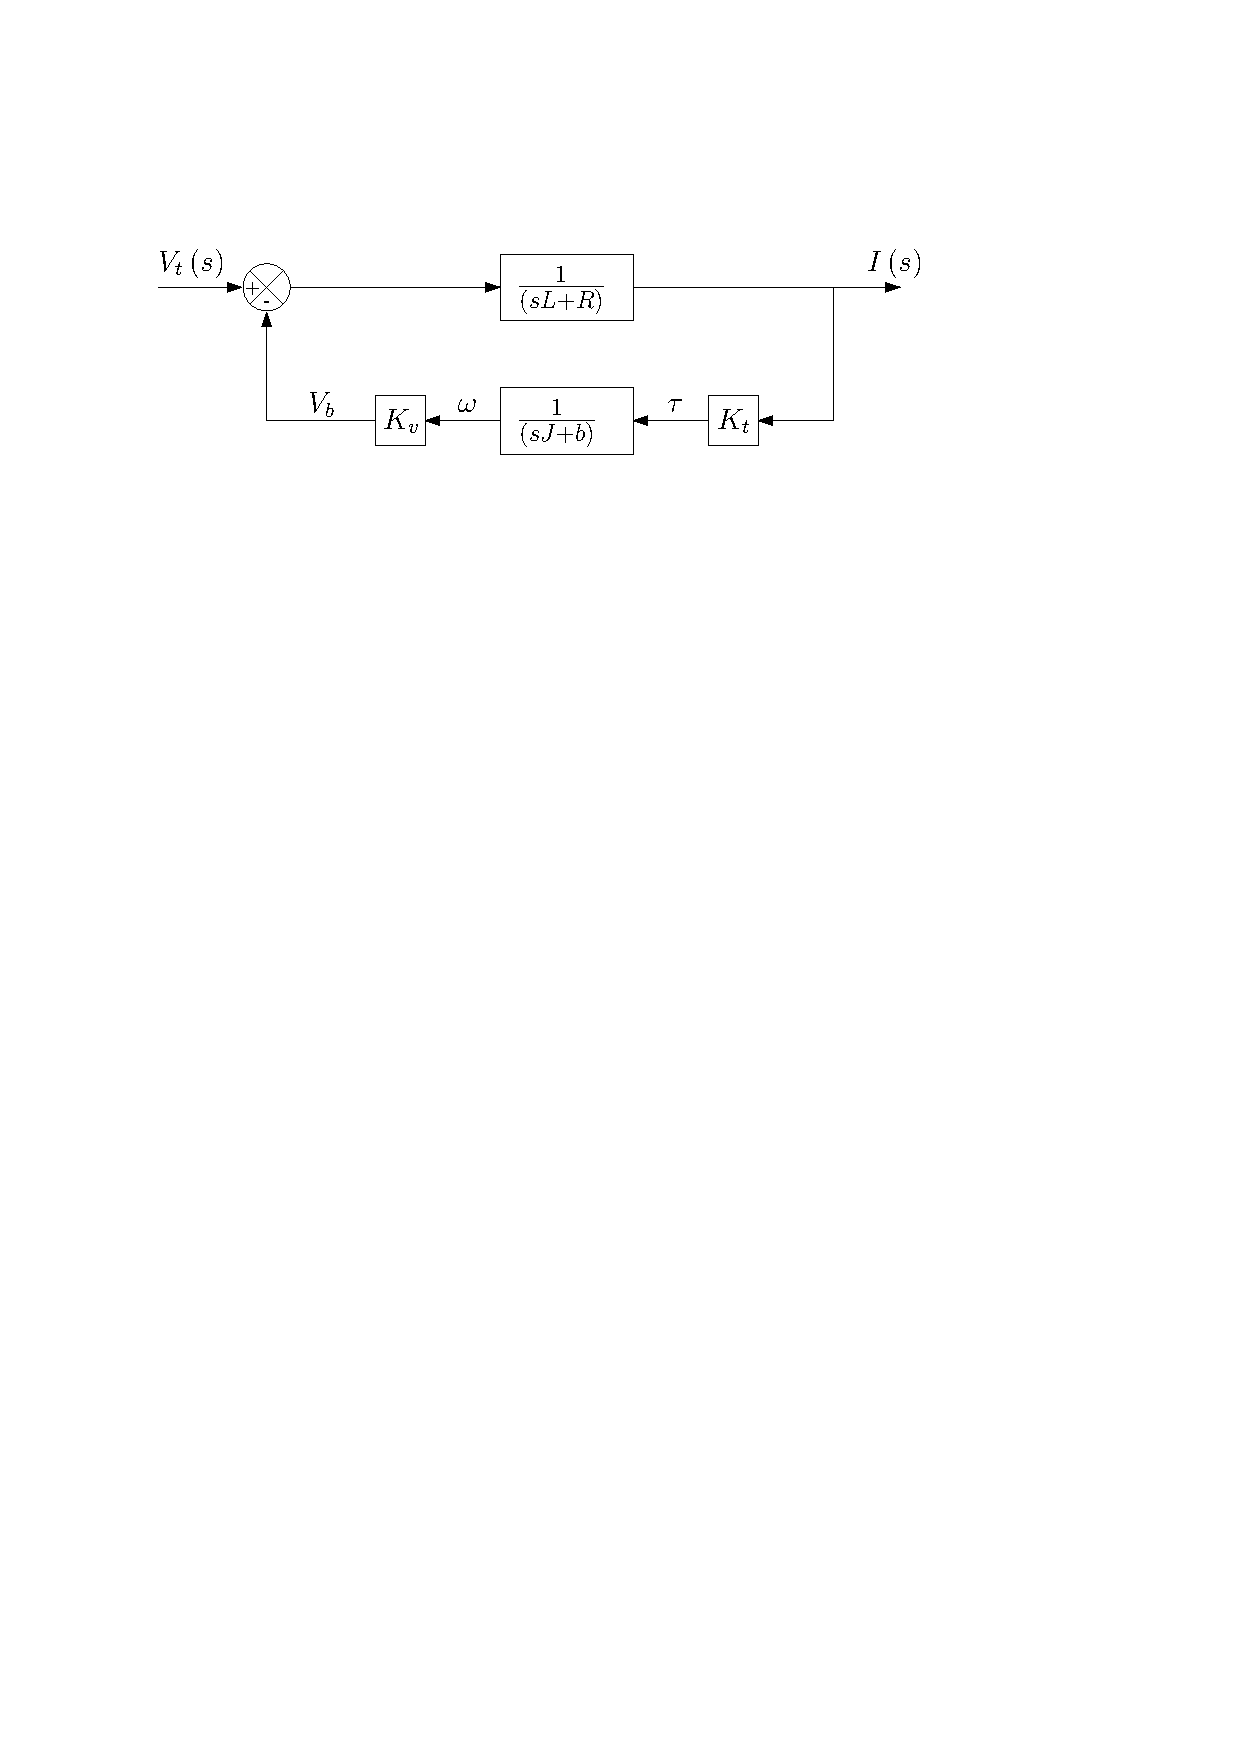
\includegraphics{dc_motor_transfer_fn}


\bibliographystyle{plain} 
\bibliography{furuta_bib}


\end{document}
